\documentclass{article}[12pt]
\usepackage{graphicx} % Required for inserting images
\usepackage{listings}
\usepackage{hyperref}
\usepackage{tabularx}
\usepackage{float}
\usepackage{subfig}

\title{EARIN Lab 3 Report}
\author{Krzysztof Rudnicki, 307585 \\ Jakub Kliszko, 303866  }
\date{\today}

\begin{document}

\maketitle

\section{Exercise Variant 2 - "Rastrigin function"}
Our task was to write a program that optimizes Rastrigin function: \\
\[ f (x, y) =
20 + (x^2 - 10 \, cos(2πx)) + (y^2 - 10 \,  cos(2πy)) \]
Using Evolutionary Strategy ($\mu$, $\lambda$) (later refered as ES($\mu$, $\lambda$)) \\ 

\section{Implementation}
Program can be ran by installing python, moving to project directory and issuing command:
\begin{lstlisting}[language=bash]
python main.py
\end{lstlisting}
There are 7 parameters we can (but do not have to) change:
\begin{enumerate}
\item Number of parents (default equal to 5)
\item Size of population (default equal to 20)
\item Mutation Strength (default equal to 0.1)
\item Number of generations (default equal to 100)
\item Minimal Value (default equal to -5.12)
\item Maximal Value (default equal to 5.12)
\item Number of outputs (default equal to 10)
\end{enumerate}
Number of outputs are strictly for displaying results and does not influence the result itself \\ 
To set parameters values user can add those flags to program run:
\begin{lstlisting}[language=bash]
    -nop --number_of_parents [number]
    -sop --size_of_population [number]
    -ms --mutation_strength [number]
    -nog --number_of_generations [number]
    -min --min_value [number]
    -max --max_value [number]
    -noo --number_of_outputs [number]
\end{lstlisting}
Order of those parameters does not matter, user can provide none, one, or any number of arguments \\ 
Exemplary use (settings all values to default values):
\begin{lstlisting}[language=bash]
    python main.py -nop 5 -sop 20 -s 0.1
    -i 100 -min -5.12 -max 5.12 -noo 10
\end{lstlisting}
There are additional flags for quality of life with the program
\begin{lstlisting}
    -nd --no_display (If used will NOT print out the plots)
    -s --save (If used WILL save plot files to code folder)
\end{lstlisting}
To print help info about program user can issue help flag:
\begin{lstlisting}[language=bash]
    python main.py -h
\end{lstlisting}
Results will be displayed on 2D scatter plot. There will be as many outputs as user wanted with incrementation of generation so that the final plot will be on final generation \\ 
\begin{figure}[H]
    \caption{Exemplary plot halfway through generation with parameters \\ nop 250 sop 1000 ms 0.1 nog 500 min max (-5.12, 5.12) noo 10 }
    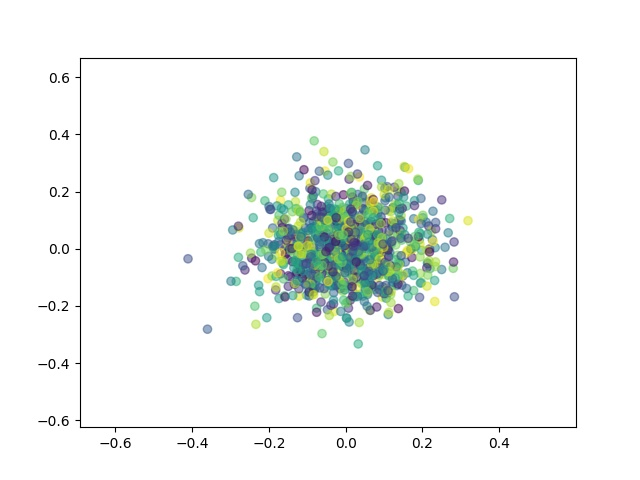
\includegraphics[width=\textwidth]{example_halfway.jpg}
    \centering
    \end{figure}
At the end summary of results on plot will display with red gradient showing results from the earliest (white) to latest (bright red) \\  
\begin{figure}[H]
    \caption{Exemplary summary plot with parameters\\ nop 250 sop 1000 ms 0.1 nog 500 min max (-5.12, 5.12) noo 10 }
    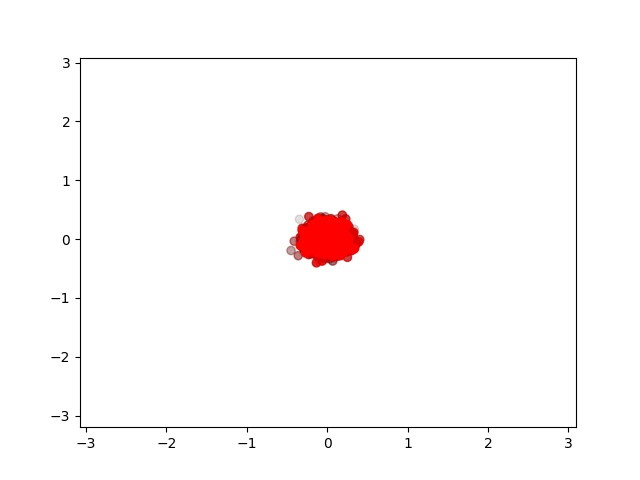
\includegraphics[width=\textwidth]{example_summary.jpg}
    \centering
    \end{figure}
Results will be displayed and if user requested saved in the same folder as code directory for further inspection, with file name containing information about input parameters \\
4 more information will also be displayed: 
\begin{itemize}
    \item Best individual found - x, y coordinates closest to 0
    \item Best fitness found
    \item Total Generation Time - including ONLY generation (not plot display)
    \item Time per generation - Total generation time divided by number of generations
\end{itemize}
\section{Results}
We have successfully implemented ES($\mu$, $\lambda$) to optimize Rastrigin function \\ 
Rastrigin function is used to test optimization algorithms as it contains a lot of local minima, our plots should therefore tend to contain values closer and closer to zeros \\ 
Exemplary run of the program with parameters:
\begin{itemize}
    \item Number of parents - 250
    \item Size of population - 1000
    \item Mutation Strength - 0.1
    \item Number of generations - 20
    \item Min value - -5.12
    \item Max value - 5.12
    \item Number of outputs - 10
\end{itemize}

\begin{figure}[H]
    \advance\leftskip-3cm
    \begin{tabular}{cc}
    \subfloat[0 generation]{
    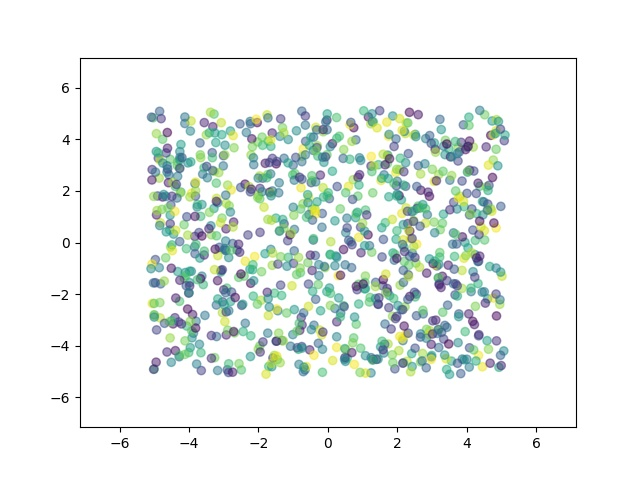
\includegraphics[width = 0.7\textwidth]{0.jpg}} &
    \subfloat[2 generation]{
    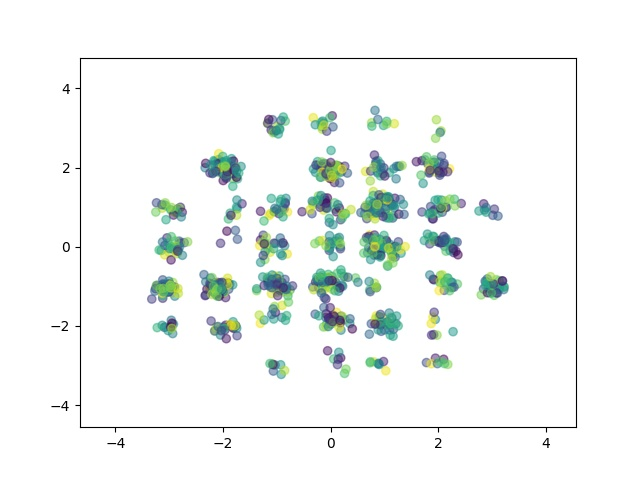
\includegraphics[width = 0.7\textwidth]{2.jpg}} \\
    \subfloat[4 generation]{
    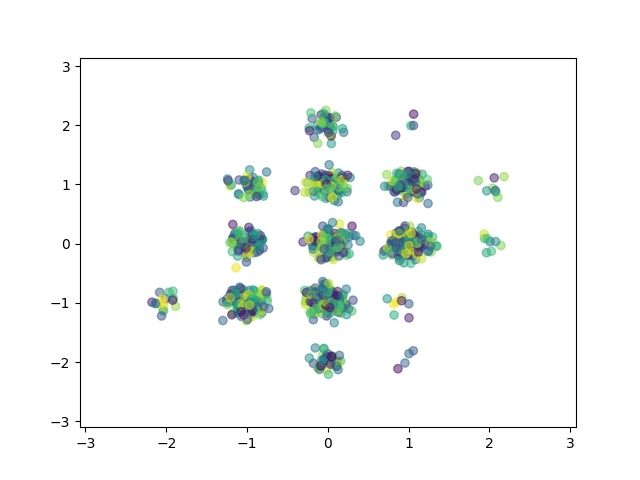
\includegraphics[width = 0.7\textwidth]{4.jpg}} &
    \subfloat[6 generation]{
    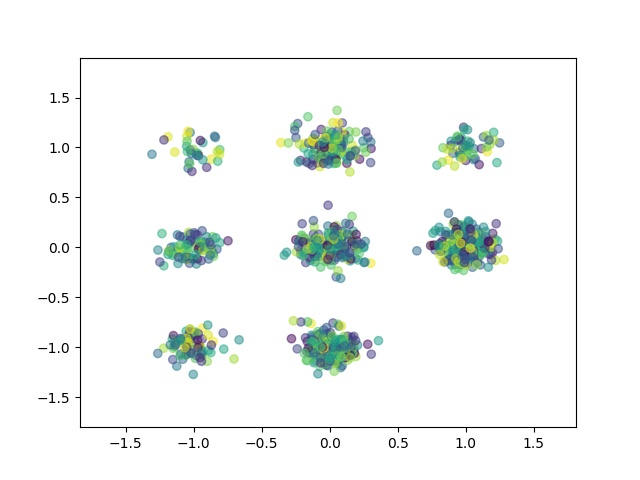
\includegraphics[width = 0.7\textwidth]{6.jpg}} \\
    \subfloat[8 generation]{
    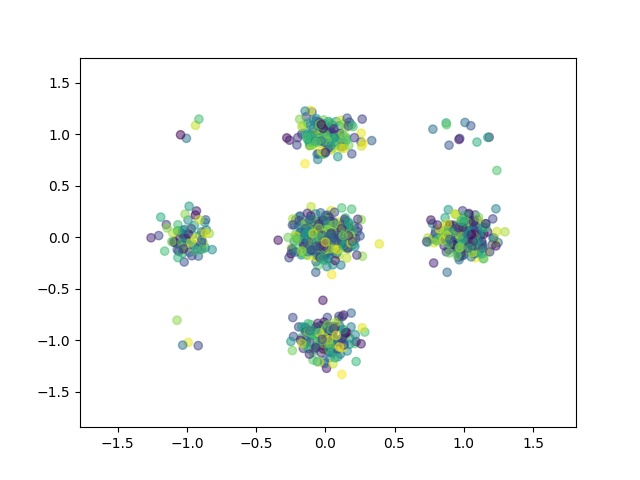
\includegraphics[width = 0.7\textwidth]{8.jpg}} &
    \subfloat[10 generation]{
    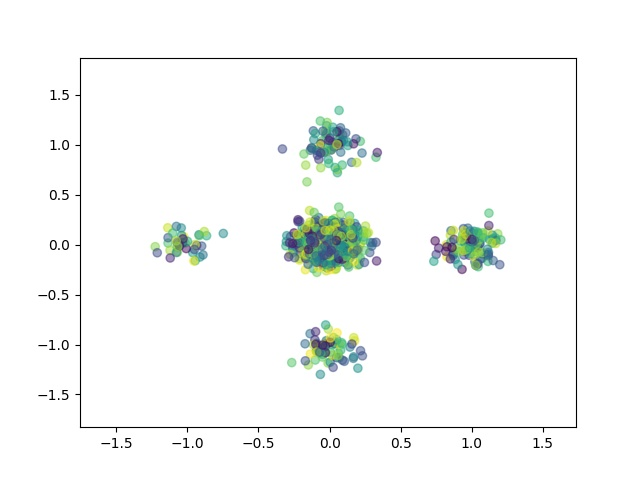
\includegraphics[width = 0.7\textwidth]{10.jpg}} \\
    \end{tabular}
\caption{First 10 Generation plots with parameters nop-250:sop-1000:ms-0.1:nog-20:min-max-(-5.12, 5.12):noo-10 }
    \end{figure}

    \begin{figure}[H]
        \advance\leftskip-3cm
        \begin{tabular}{cc}
    
        \subfloat[12 generation]{
        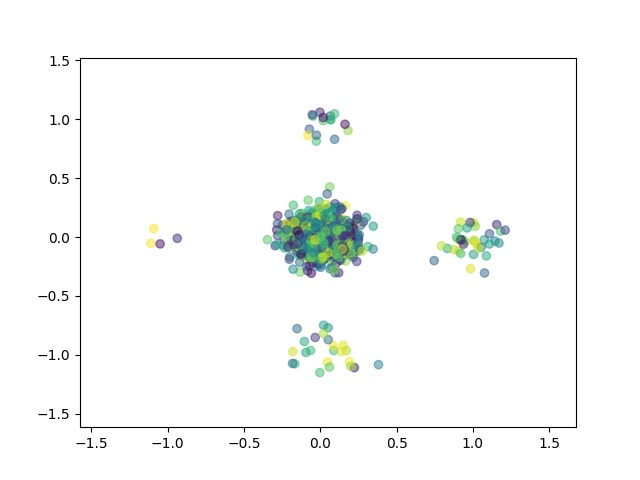
\includegraphics[width = 0.7\textwidth]{12.jpg}} &
        \subfloat[14 generation]{
        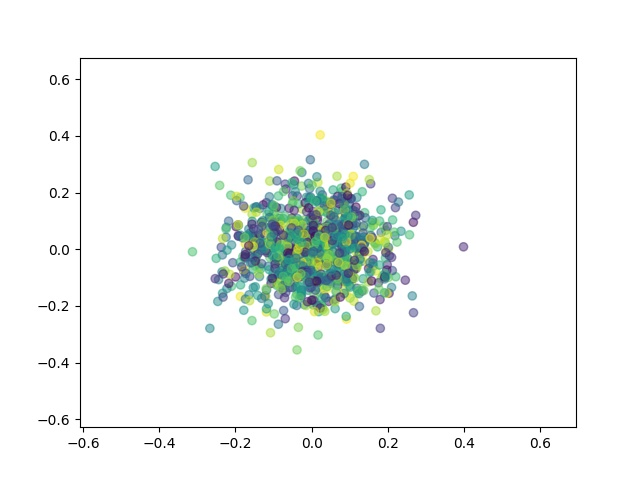
\includegraphics[width = 0.7\textwidth]{14.jpg}} \\
        \subfloat[16 generation]{
        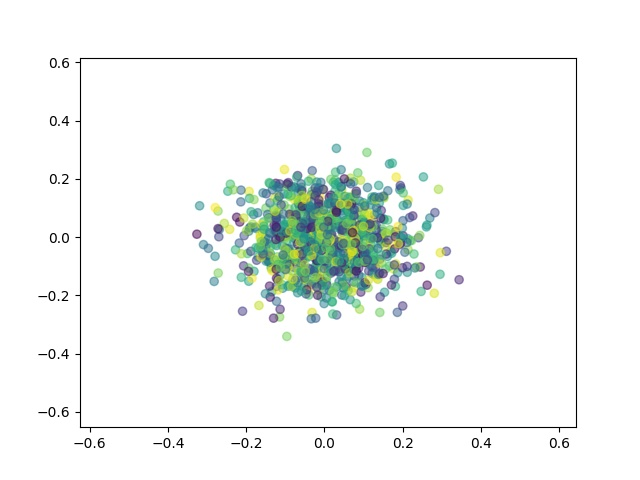
\includegraphics[width = 0.7\textwidth]{16.jpg}} &
        \subfloat[18 generation]{
        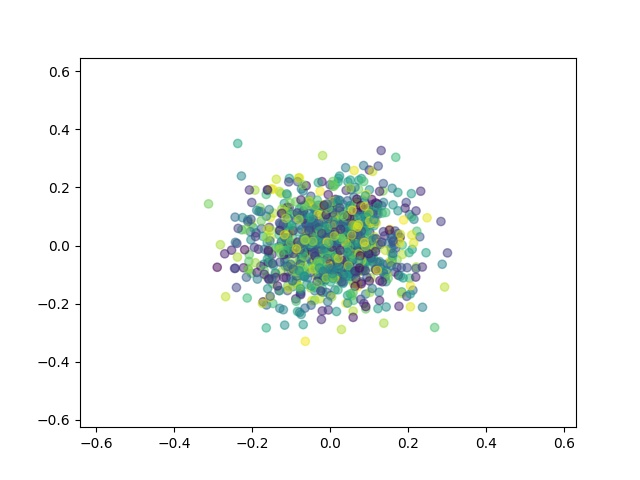
\includegraphics[width = 0.7\textwidth]{18.jpg}} \\
        \subfloat[20 generation]{
        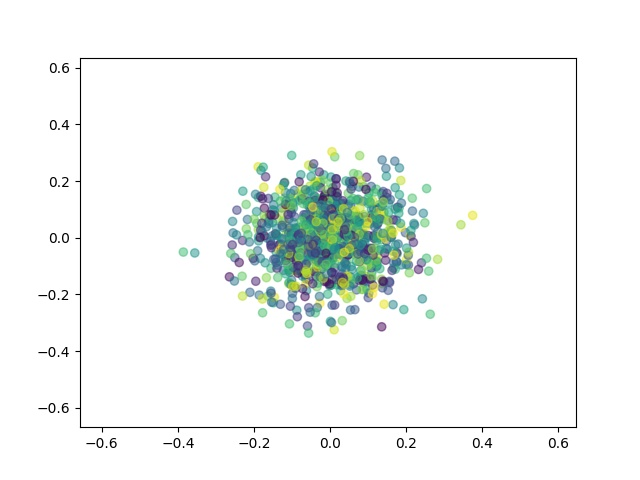
\includegraphics[width = 0.7\textwidth]{20.jpg}} &
        \subfloat[Summary]{
        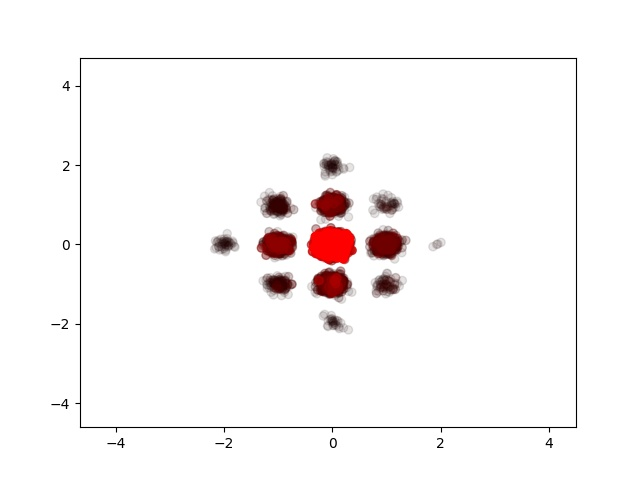
\includegraphics[width = 0.7\textwidth]{summary.jpg}} \\
        \end{tabular}
    \caption{Last 10 Generation plots and summary plot with parameters nop-250:sop-1000:ms-0.1:nog-20:min-max-(-5.12, 5.12):noo-10 }
        \end{figure}

As we can see with every generation the result comes closer and closer to the center of the plot (point (0, 0)) \\ At the begining (0 generation) we have random points with coordinates between -5.12 and 5.12 \\ Which later form groups of points with center group becoming bigger and bigger (generations between 2 and 12) \\ To finallly reach one big group centered around (0, 0) (generations between 14 and 20) \\ Summary plot clearly shows that the final groups (once that most red) are close to point (0, 0) \\ 
Additonal info from execution of the program with those parameters: 
\begin{itemize}
    \item Best individual found: [-0.00512557 -0.00185114]
    \item Best fitness found: 0.005891436754870583
    \item Total generation time:  0.0532705290006561
    \item Time per generation:  0.0026635264500328047
\end{itemize}


\end{document}
